\documentclass[11pt,answers]{exam}
\usepackage[legalpaper,bindingoffset=0in,left=.6in,right=0.8in,top=0.4in,bottom=0.7in,headsep=.5\baselineskip]{geometry}
\usepackage[utf8]{inputenc}
\usepackage{graphicx}
\usepackage{listings}
\usepackage{enumitem}
\usepackage{amsmath}
\usepackage{multirow}
\usepackage{multicol}
\usepackage{caption}
\usepackage{tabularx}
\usepackage{url}
\usepackage{amssymb}
\usepackage{array}
\usepackage{tikz}
\usepackage{graphicx}
\usetikzlibrary{shapes.callouts, positioning, arrows.meta, shapes.geometric, shadows, calc, patterns, 3d, backgrounds, shadings}
\usepackage{adjustbox}
\usepackage{ragged2e}
\usepackage{pgfplots}

%\pagenumbering{gobble}
\def\changemargin#1#2{\list{}{\rightmargin#2\leftmargin#1}
\item[]}
\let\endchangemargin=\endlist
\usepackage{xcolor}
\usepackage{listings}
\definecolor{mGreen}{rgb}{0,0.6,0}
\definecolor{mGray}{rgb}{0.5,0.5,0.5}
\definecolor{mPurple}{rgb}{0.58,0,0.82}
\definecolor{backgroundColour}{rgb}{0.95,0.95,0.92}
\lstset{
  language=C,
  basicstyle=\ttfamily\small,
  aboveskip={1.0\baselineskip},
  belowskip={1.0\baselineskip},
  columns=fixed,
  extendedchars=true,
  breaklines=true,
  tabsize=4,
  prebreak=\raisebox{0ex}[0ex][0ex]{\ensuremath{\hookleftarrow}},
  frame=lines,
  showtabs=false,
  showspaces=false,
  showstringspaces=false,
  keywordstyle=\color[rgb]{0.627,0.126,0.941},
  commentstyle=\color[rgb]{0.133,0.545,0.133},
  stringstyle=\color[rgb]{01,0,0},
  numbers=left,
  numberstyle=\small,
  stepnumber=1,
  numbersep=10pt,
  captionpos=t,
escapeinside={\%*}{*)}
}
%\renewcommand\thequestion{Q.\arabic{question}}
%\renewcommand{\questionlabel}{\thequestion)}
%\renewcommand{\questionshook}{%
%\setlength{\leftmargin}{0pt}%
%\setlength{\labelwidth}{-\labelsep}%
%}

%\pointsinrightmargin
\pointsdroppedatright
%\marksnotpoints
%\marginpointname{ \points}
%\pointformat{\boldmath\themarginpoints}

\title{
\begin{changemargin}{0.68cm}{0.68cm}
  \normalsize Class Test 3\hfill {January 2025}\\
\end{changemargin}
\vspace{.4cm}
\large BANGLADESH UNIVERSITY OF ENGINEERING AND TECHNOLOGY\\
\vspace{.1cm}
Department of Computer Science and Engineering\\
\vspace{.2cm}
L-4/T-1 \hspace{.1cm} CSE 409: Computer Graphics\\
\vspace{.2cm}
\textbf{Time: 25 minutes} \hspace{2.2cm} \textbf{Marks: 20}
\begin{changemargin}{0.68cm}{0.68cm}
  \normalsize Student Name: \underline{\hspace{6.5cm}} \hfill Student ID: \underline{\hspace{2.5cm}}\\
\end{changemargin}
}
\author{}
\date{}

\begin{document}

\maketitle
\thispagestyle{empty}
\begin{questions}
\vspace{-2cm}

\question[]{
a) What happens if we shoot rays from light sources instead of the eye?
\hfill (2) \\

\vspace*{3cm}

b) For a 3840$\times$2160 resolution image, how many rays should be cast (at least) for a ray-traced image?
\hfill (2) \\

\vspace*{3cm}

c) During calculations, how do we ensure that we take the closest intersection?
\hfill (2)

\vspace*{3cm}
}
\question[]
{
\begin{multicols}{2}
a) In the triangle $ABC$ what is the barycentric
\mbox{coordinates} $(\alpha, \beta, \gamma)$ of point $P$? \\
$AB=AC=5$ and $\angle CAP = 30^\circ, \angle PAB = 45^\circ$. \\
(Hint: $\text{area} = \frac{1}{2} ab \sin{\theta}$)
\vfill
\columnbreak
\centering
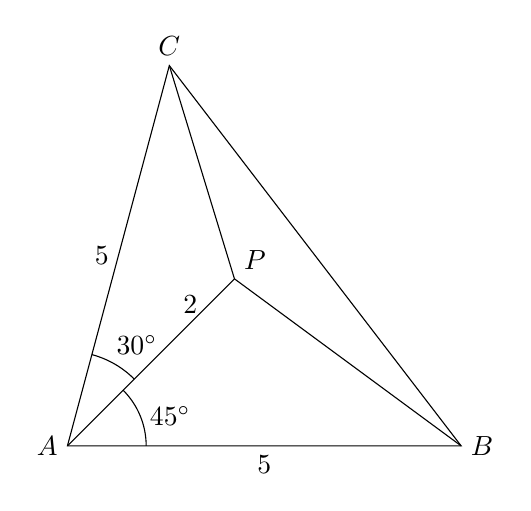
\begin{tikzpicture}
\coordinate (A) at (0, 0);
\coordinate (B) at (0:5);
\coordinate (C) at (75:5);
\coordinate (P) at (45:3);
\draw (A) node[left] {$A$}  -- node[midway,below] {$5$} (B) node[right] {$B$} -- (C) node[above] {$C$} -- node[midway,left] {$5$} cycle;
\draw (A) -- (P) node[midway, above, shift={(0.5,0.5)}] {$2$};
\draw (B) -- (P) node[above right] {$P$};
\draw (C) -- (P);
\draw (1,0) arc [start angle=0, end angle=45, radius=1cm]
node[midway, right] {$45^{\circ}$};
\draw (45:1.2) arc [start angle=45, end angle=75, radius=1.2cm]
node[midway, above right,xshift=-0.1cm] {$30^{\circ}$};
\end{tikzpicture}
\hfill (4)
\end{multicols}

\vspace*{5cm}
b) If the vertices $A$, $B$ and $C$ are to be coloured red (255, 0, 0), green (0, 255, 0) and blue (0, 0, 255) respectively, what would be the interpolated colour of $P$ in RGB? \hfill (2)

\vspace*{2cm}
}
\newpage
\question[]
{
\begin{multicols}{2}

a) A highly aggressive alien race shot their laser canon towards earth. It
already destroyed the aesteroid A3205 in the solar system. Will earth \mbox{survive}?
Radius of earth is 6400 KM. All units in $10^6$ meters.

\vfill
\columnbreak
\centering
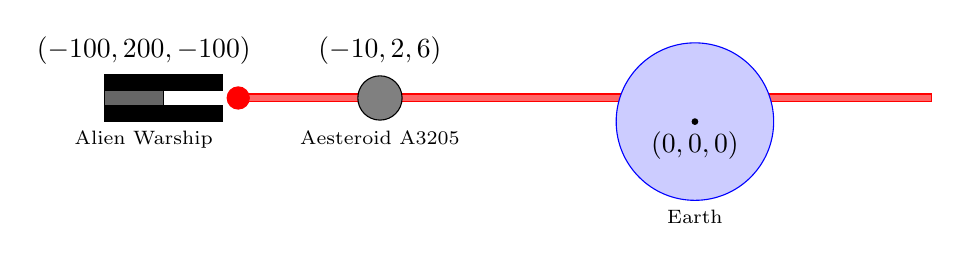
\begin{tikzpicture}
% spaceship
\draw[black,fill=black!60] (-7.5,0.4) rectangle (-6.75,0.2);
\draw[black,fill=black] (-7.5,0) rectangle (-6,0.2);
\draw[black,fill=black] (-7.5,0.4) rectangle (-6,0.6);
\node[below] at (-7, 0.0) {\scriptsize Alien Warship};
\node[above] at (-7, 0.6) {$(-100, 200, -100)$};
% laser
\draw[red,fill=red!60] (-5.9, 0.25) rectangle (3,0.35);
\draw[red,fill=red] (-5.8,0.3) circle (4pt);
% earth
\draw[blue,fill=blue!20] (0,0) circle (1cm) node[below] {};
\draw[black,fill=black] (0,0) circle (1pt) node[below] {$(0,0,0)$};
\node[below] at (0,-1) {\scriptsize Earth};
% aesteroid
\draw[black,fill=black!50] (-4,0.3) circle (8pt) node[below, yshift=-0.3cm]
{\scriptsize Aesteroid A3205} node[above, yshift=0.3cm] {$(-10, 2, 6)$};

\end{tikzpicture}
\end{multicols}
\hfill (4)

\vspace{16cm}

b) If earth survives, by how far did the laser miss? If not, at what distance from the Alien Warship did the laser hit earth?
\hfill (2)
}
\vspace{8cm}
\question[]For your hard work and attending the exam so early in the morning.\hfill (2)

\end{questions}
\end{document}